% Archivo generado automáticamente con los problemas
\section*{Problems}
Sección: 7_Feynman_rules
Páginas: 122-125
Contenido:
7.1 Consider the Lagrangian for φ3 theory,
L = −1
2φ(□+ m2)φ + g
3!φ3.
(7.122)
(a) Draw a tree-level Feynman diagram for the decay φ →φφ. Write down the
corresponding amplitude using the Feynman rules.
(b) Now consider the one-loop correction, given by
φ
φ
φ
(7.123)
Write down the corresponding amplitude using the Feynman rules.
(c) Now start over and write down the diagram from part (b) in position space,
in terms of integrals over the intermediate points and Wick contractions,
represented with factors of DF .
(d) Show that after you apply LSZ, what you got in (c) reduces to what you got
in (b), by integrating the phases into δ-functions, and integrating over those
δ-functions.

7.2 Calculate the contribution to 2 →4 scattering from the Lagrangian L = −1
2φ□φ+
g
3!φ3 + 1
6!λφ6 from both the connected diagram, with the 6-point vertex, and the
disconnected diagram with the 3-point vertex. Show that there is no interference
between the two diagrams. (There are of course many connected diagrams with the
3-point vertex that you can ignore.)

7.3 Non-relativistic Møller scattering: e−e−→e−e−. If the electron and photon were
spinless, we could write the Lagrangian as
L = −1
2φe(□+ m2
e)φe −1
2A0□A0 + emeA0φeφe,
(7.124)
where A0 is the scalar potential and the factor of me comes from the non-relativistic
limit as in Section 5.2 (or by dimensional analysis!).
104
Feynman rules
(a) Draw the three tree-level e−e−
→e−e−diagrams following from this
Lagrangian.
(b) Which one of the diagrams would be forbidden in real QED?
(c) Evaluate the other two diagrams, and express the answers in terms of s, t and u.
Give the diagrams an extra relative minus sign, because electrons are fermions.
(d) Now let us put back the spin. In the non-relativistic limit, the electron spin is
conserved. This should be true at each vertex, since the photon is too soft to
carry off any spin angular momentum. Thus, a vertex can only allow for |↑⟩→
|↑; γ⟩or |↓⟩→|↓; γ⟩. This forbids, for example, |↑↓⟩→|↑↑⟩from occurring.
For each of the 16 possible sets of spins for the four electrons (for example
|↑↓⟩→|↑↑⟩), which processes are forbidden, and which get contributions from
the s-, t- or u-channels?
(e) It is difficult to measure electron spins. Thus, assume the beams are unpo-
larized, meaning that they have an equal fraction of spin-up and spin-down
electrons, and that you do not measure the final electron spins, only the scat-
tering angle θ. What is the total rate
dσ
d cos θ you would measure? Express the
answer in terms of ECM and θ. Sketch the angular distribution.

7.4 We made a distinction between kinetic terms, which are bilinear in fields, and inter-
actions, which have three or more fields. Time evolution with the kinetic terms is
solved exactly as part of the free Hamiltonian. Suppose, instead, we only put the
derivative terms in the free Hamiltonian and treated the mass as an interaction. So,
H0 = 1
2φ□φ,
Hint = 1
2m2φ2.
(7.125)
(a) Draw the (somewhat degenerate looking) Feynman graphs that contribute to
the 2-point function ⟨0|T{φ(x)φ(y)}|0⟩using only this interaction, up to
order m6.
(b) Evaluate the graphs.
(c) Sum the series to all orders in m2 and show you reproduce the propagator that
would have come from taking H0 = 1
2φ□φ + 1
2m2φ2.
(d) Repeat the exercise classically: Solve for the massless propagator using an
external current, perturb with the mass, sum the series, and show that you get
the same answer as if you included the mass to begin with.

7.5 Show in general that integrating by parts does not affect matrix elements.

7.6 Use the Lagrangian
L = −1
2φ1□φ1 −1
2φ2□φ2 + λ
2 φ1(∂μφ2)(∂μφ2) + g
2φ2
1φ2
(7.126)
to calculate the differential cross section
dσ
dΩ(φ1φ2 →φ1φ2)
(7.127)
at tree level.

7.7 Consider a Feynman diagram that looks like a regular tetrahedron, with the external
lines coming out of the four corners. This can contribute to 2 →2 scattering in a
scalar field theory with interaction λ
4!φ4. You can take φ to be massless.
Problems
105
(a) Write down the corresponding amplitude including the appropriate symmetry
factor.
(b) What would the symmetry factor be for the same diagram in φ3 theory without
the external lines?

7.8 Radioactive decay. The muon decays to an electron and two neutrinos through an
intermediate massive particle called the W −boson. The muon, electron and W −
all have charge −1.
(a) Write down a Lagrangian that would allow for μ−→e−¯νeνμ. Assume the W
and other particles are all scalars, and the e−, νe and νμ are massless. Call the
coupling g.
(b) Calculate |M|2 for this decay in the limit that the W mass, mW , is large.
(c) The decay rate Γ (=
1
lifetime) is proportional to |M|2. The coupling g should
be dimensionless (like the coupling e for the photon), but appears dimension-
ful because we ignore spin. If the W spin were included, you would get extra
factors of pμ, which would turn into a factor of √s = mμ in |M|2. Use dimen-
sional analysis to figure out what power of mμ should be there. Also, throw in
a
1
192π3 for the three-body phase space, as in Eq. (5.55) from Problem 5.3.
(d) Pick some reasonable perturbative value for g and use the muon mass
(mμ = 105 MeV) and lifetime (2.2 × 10−6 s) to estimate the W mass.
(e) The tauon, τ, also decays to e−νeνμ. Use the τ lifetime Γ−1
tot = 2.9 × 10−13 s
and previous parts to estimate the τ mass. Which of mW , g, mμ, the muon
lifetime, or the 192π3 we threw in does your prediction depend on?
(f) In reality, the tauon only decays as τ →e−νeνμ 17.8% of the time. Use this
fact to refine your τ mass estimate.
(g) How could you measure g and MW separately using very precise measure-
ments of the μ and τ decay distributions? What precision would you need
(in %)?

7.9 Unstable particles. Unstable particles pick up imaginary parts that generate a width
Γ in their resonance line shape. This problem will develop an understanding of
what is meant by the terms width and pick up.
(a) What would the cross section be for s-channel scattering if the intermediate
propagator were
i
p2−m2+imΓ, where Γ > 0? This is called the Breit–Wigner
distribution.
(b) Sketch the cross section as a function of x =
s
m2 for Γ
m small and for Γ
m large.
(c) Show that a propagator only has an imaginary part if it goes on-shell. Explicitly,
show that Im(M) = −πδ(p2 −m2), when iM =
i
p2−m2+iε.
(d) Loops of particles can produce effective interactions that have imaginary parts.
Suppose we have another particle ψ and an interaction φψψ in the Lagrangian.
Loops of ψ will have imaginary parts if and only if ψ is lighter than half of φ,
that is, if φ →ψψ is allowed kinematically. Draw a series of loop corrections
to the φ propagator. Show that, if these give an imaginary number, you can sum
the graphs to reproduce the propagator in part (a).
(e) What is the connection between parts (c) and (d)? Can you see why the width
is related to the decay rate?

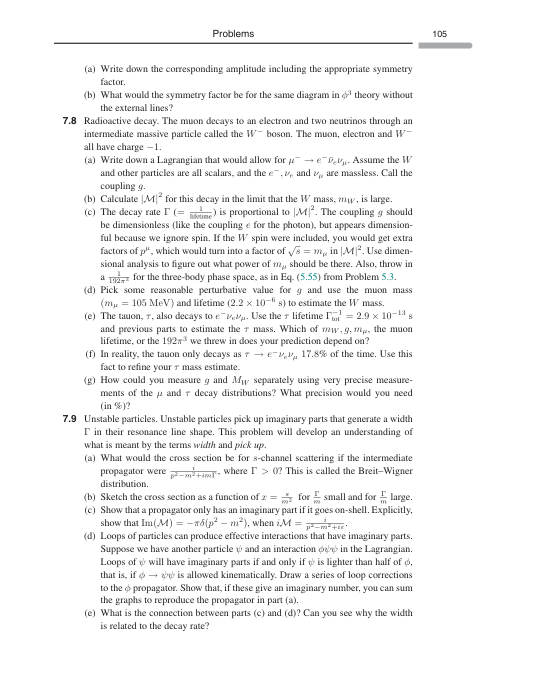
\includegraphics{./figs/7_Feynman_rules_page_125.png}

---

